%Empieza configuracion de capitulo
\setstretch{1.0}
\titleformat{\chapter}[block]{\Large\bfseries}{CHAPTER \Huge\thechapter\vspace{25 pt}}{0 pt}{\\\fontsize{26}{36}\selectfont}
\titlespacing{\chapter}{0 pt}{30 pt}{50 pt}[0 pt]
\titleformat{\section}{\Large\bfseries}{\thesection}{0 pt}{\hspace{30 pt}}
\titleformat{\subsection}{\large\bfseries}{\thesubsection}{0 pt}{\hspace{30 pt}}
\pagestyle{fancy}
\fancyhead[LO,LE]{\footnotesize\emph{\leftmark}}
\fancyhead[RO,RE]{\thepage}
\fancyfoot[CO,CE]{}
%Termina configuracion de capitulo

\chapter{System Architecture}
\setstretch{1.5} %Regresa el interlineado a 1.5

\normalsize
\noindent
In this chapter we will cover the architecture of the system, from a hardware
and software perspective. As well as the MPI implementation in Yocto. There is
a brief description of the benchmarks (with the fixes implemented). In the end
we present the description of the topology implemented

\section{Embedded System}
\noindent

As we described in the theoretical framework an embedded system is some
combination of computer hardware and software, either fixed in capability or
programmable, that is specifically designed for a particular function. We will
describe hardware of the development board as well as the software we are going
to use (operating system and firmware).

\subsection{Development Board} The platform we will use for our experiment is the
Intel \makeatletter @  Atom-TM Processor E3825. Their main characteristics are
described in (table~\ref{tab:4.1}).\cite{E3825}:

    \begin{center}
    \rowcolors{1}{gray}{white}
    \begin{tabular}{ | l | r |}
        \hline
        Processor Number & E3825  \\ \hline
        \# of cores & 2  \\ \hline
        \# of Thread & 2  \\ \hline
        Clock Speed & 1.3 GHz  \\ \hline
        L2 Cache & 1MB  \\ \hline
        Instruction Set & 64 bit  \\ \hline
    \end{tabular}
    \captionof{table}{Intel Atom Processor E3825
    Especificaciones} \label{tab:4.1}
    \end{center}

The comercial name of this platform is Minnowboard Max.  figure~\ref{fig:4.1}
and  figure~\ref{fig:4.2} This is a development platform for both
professionals and makers. Minnowboard Max is an open hardware platform, The
concept of ''open-source hardware'' or ''open hardware'' is not yet as well
known or widespread as the free software or open-source software concept.
However, it shares the same principles: anyone should be able to see the source
(the design documentation in case of hardware), study it, modify it and share
it.\cite{CERN}

\begin{figure}[H]
\centering
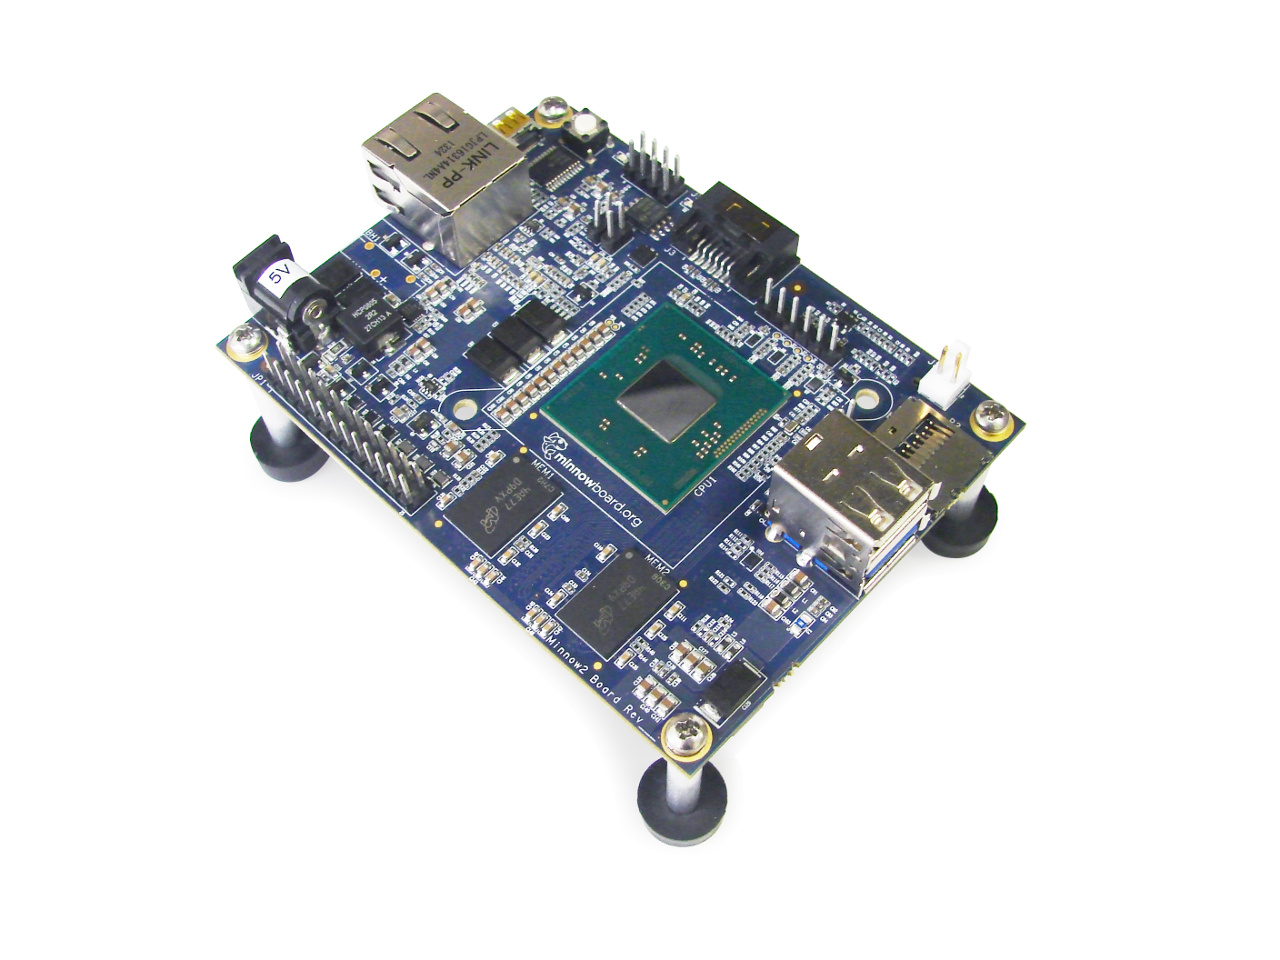
\includegraphics[width=0.75\textwidth]{images/minnow-max.jpg}.png
\caption{The Minnowboard Max}
\label{fig:4.1}
\end{figure}


\begin{figure}[H]
\centering
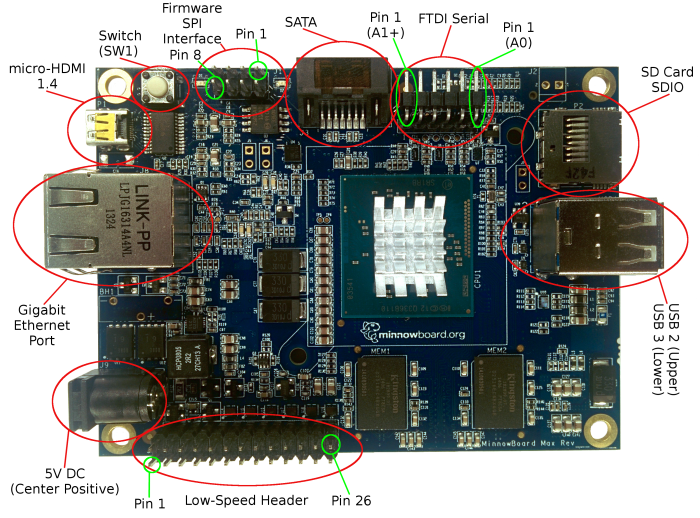
\includegraphics[width=0.75\textwidth]{images/minnow-max-2.png}
\caption{Conection Ports of the Minnowboard Max}
\label{fig:4.2}
\end{figure}

\subsection{Embedded Operating System} 

In order to perform the experiments we need a full Opearting System running on
the developemnt board. This means that it will require a boot manager, a full
file system , kernel and user space.  As we saw on the theoretical framework is
hard to have such thing from scratch, instead of that we have Yocto project.
Yocto project is designed to create a full Linux OS for embedded platforms.
However there are other ways to boot an OS, either a custom OS from scratch or
a generic one as Fedora. We will need to experiment which one is better for our
needs.

\section{Message Passing Interface (MPI) implementation}
\noindent

The Message Passing Interface Standard (MPI) is a message passing library
standard based on the consensus of the MPI Forum, which has over 40
participating organizations, including vendors, researchers, software library
developers, and users. The goal of the Message Passing Interface is to
establish a portable, efficient, and flexible standard for message passing
that will be widely used for writing message passing programs. MPI is not an IEEE
or ISO standard, but has in fact, become the "industry standard" for writing
message passing programs on HPC platforms. 

The implementation we are going to test are : 

\begin{itemize}
    \item Fedora version
    \item Clear Linux for Intel Architecture version
    \item Yocto version (ported by Victor Rodriguez)
\end{itemize}

The diversity of version help us to create a better support to chose
optimizations on the experiments. If we just choose an OS without proves that
this one is the better for what we want, we will end having bottle necks , the
same that industry had 20 years ago to say that an embedded distributed
platform is not possible.

\section{Benchmarks}
\noindent

High-performance computing (HPC) is a broad term that at its core represents
compute intensive applications that need acceleration. Users of application
acceleration systems range from medical imaging, financial trading, oil and gas
expiration, to bio science, data warehousing, data security, and many more. In
the information age, the need for acceleration of data processing is growing
exponentially and the markets deploying HPC for their applications are growing
every day. The HPC expansion is being fueled by the co-processor, which is
fundamental to the future of HPC. (High- Performance Computing Applications)

Our main scope will be to find which HPC applications better suit a distributed
dedicated approach and topology.
In order to make a fare comparison of the multiple topologies we will implement
against an HPC server (Intel Xeon) we will use the HPC Challenge Benchmark. The
HPC Challenge Benchmark is a set of benchmarks targeting to test multiple
attributes that can contribute substantially to the real- world performance of
HPC systems, co-sponsored by the DARPA High Productivity Computing Systems
program, the United States Department of Energy and the National Science
Foundation. (Dongarra)

The HPC Challenge benchmark consists of basically 7 tests:


\begin{itemize}
    \item HPL - the Linpack TPP benchmark which measures the floating point
    rate of execution for solving a linear system of equations.
    \item DGEMM - measures the floating point rate of execution of double
    precision real matrix- matrix multiplication.
    \item STREAM - a simple synthetic benchmark program that measures sustainable
    memory bandwidth (in GB/s) and the corresponding computation rate for
    simple vector kernel.
    \item PTRANS (parallel matrix transpose) - exercises the communications where
    pairs of processors communicate with each other simultaneously. It is a useful test
    of the total communications capacity of the network. 
    \item RandomAccess - measures the rate of integer random updates of memory
    (GUPS).
    \item FFT - measures the floating point rate of execution of double precision
    complex one dimensional Discrete Fourier Transform (DFT).
    \item Communication bandwidth and latency - a set of tests to measure latency
    and bandwidth of a number of simultaneous communication patterns; based on beff
    (effective bandwidth benchmark).
\end{itemize}



\section{Topologies}
\noindent

\clearpage
